\chapter{Gait Watch and Qualisys Optica motion tracker}
\label{ch:GWandQS}

\section{Introduction and chapter's structure}
After explaining and comparing both systems Gait Watch and Force Plate, we proceed now to do analysis of te differences and similarities between Gait Watch and Qualisys Optical motion tracker.

It has been demonstrated that Qualisys System is a accurate system to analyse the body movements and it can be used in several applications. However, this system has a lot of constraints like the possibility of application scope.

Thus, we are going to do a comparison with Gait Watch system, a system based in inertial sensors being more potable and cheaper.
Along this chapter we will explain how the pitch has been calculated using Qualisys System. This will be what we will compare with the angles obtained through inertial sensors.


\section{Computing Euler angles using Qualisys System}
To compute the Euler angle, the subject is wearing two infrared markers per segment placed in both thighs and shanks. The infrared optical cameras emit infrared light and this reflects in the markers placed over the body allowing to know the position of the markers.

The pitch angle of such segment is computed between the vector defined by the upper and lower markers and the vector normal to the Earth’s surface. To be able to compute it we first have to define a third point which has the same X coordinate as the lower marker and the same Z coordinate as the upper marker. This will define a right triangle in which one of the contiguous cathetus is normal to the Earth’s surface and the hypotenuse is defined by the line between the upper and the lower point. Therefore, by calculating the arctangent we can easily find the angle of the right triangle, which is, in turn, the pitch angle\cite{OlivaresBotzel2013}. We can see this in \ref{fig:pitchQS}

\begin{figure}[H]
	\centering
	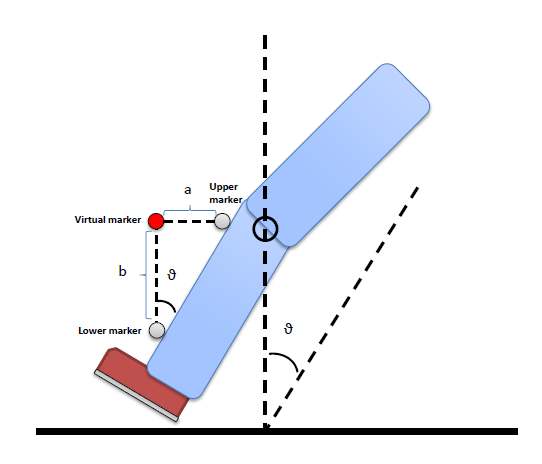
\epsfig{file=imagenes/pitchQS, width=7cm}
	\caption{Diagram of the pitch computation using the Qualisys System \cite{OlivaresBotzel2013}.}
	\label{fig:pitchQS}
\end{figure}

Thus, the pitch angle is computed as follows:

\begin{equation}
\label{angleQS1}
	\theta_{QS}= arctang(\frac{a}{b})
\end{equation}

\begin{equation}
\label{angleQS2}
	a= \sqrt{(x_{upper}-x_{lower})^{2} + (z_{upper}-z_{upper})^{2} }
\end{equation}

\begin{equation}
\label{angleQS3}
	b= \sqrt{(x_{lower}-x_{lower})^{2} + (z_{lower}-z_{upper})^{2} }
\end{equation}

where $ [x_{lower}, z_{lower} ] $ and $ [x_{upper}, z_{upper} ] $ are the coordinates of the projections of the lower an upper markers in the XZ plane, respectively.

\section{Feature extraction}

\section{Results discurssion}

